\documentclass[12pt]{article}
\usepackage{url, graphicx}
\usepackage{geometry}
\usepackage{amsmath}
\usepackage{fancyhdr}
\usepackage{nopageno}
\usepackage[usenames, dvipsnames]{color}

\pagestyle{fancy}

\title{\huge Lecture 8: Graph Algorithms: Breadth First Search}
\author{}
\date{}
\pagestyle{fancy}
\fancyhf{}
\lhead{COMP 251 Winter 2018}
\rhead{Lecture 8}
\lfoot{$24^{th}$ Jan, 2018}
\rfoot{\copyright{}Yutong Yan}
\newcommand{\forceindent}{\leavevmode{\parindent=1em\indent}}
\begin{document}
\maketitle


\section{Graph Exploration}
\renewcommand{\labelitemii}{$\circ$}
\renewcommand{\labelitemiii}{$\cdot$}
\renewcommand{\labelitemiii}{$\rightarrow$}
\renewcommand{\labelitemiv}{$\star$}
\begin{itemize}
\item Given a graph and two specified vertices r and v, a fundamental question is:
	\begin{itemize}
	\item Does the graph contain a path from r to v?
	\end{itemize}
\item In fact, given a root vertex r, we will be able to answer this question \underline{simultaneously} for all non-root vertices.
\item That is, we can efficiently determine which vertices are reachable by \textbf{path traversal} starting at the root vertex.
\end{itemize}

\section{Search Applications}
\renewcommand{\labelitemii}{$\circ$}
\renewcommand{\labelitemiii}{$\cdot$}
\renewcommand{\labelitemiii}{$\rightarrow$}
\renewcommand{\labelitemiv}{$\star$}
\begin{itemize}
\item Graph Search has a \textbf{vast} number of applications.
\item These can be simple applications:
	\begin{itemize}
	\item How do we explore a maze?
	\item How do I travel from Montreal to Toronto?
	\end{itemize}
\item Or, they can be much more substantive.
	\begin{itemize}
	\item What is the best way to search the web?
	\item How, and how far, will a disease spread through the population?
	\end{itemize}
\end{itemize}



\section{The Generic Search Algorithm}
\renewcommand{\labelitemii}{$\circ$}
\renewcommand{\labelitemiii}{$\cdot$}
\renewcommand{\labelitemiii}{$\rightarrow$}
\renewcommand{\labelitemiv}{$\star$}
\begin{itemize}
\item The Generic Search Algorithm:\\
\\
\underline{The Search Algorithm}\\
Put r into a bag\\
\forceindent \textbf{While} the bag is non-empty\\
\forceindent \forceindent Remove v from the bag\\
\forceindent \forceindent If v is unmarked \\
\forceindent \forceindent \forceindent Mark v\\
\forceindent \forceindent \forceindent For each arc(v,w)\\
\forceindent \forceindent \forceindent \forceindent Put w into the bag
\item Formal pseudocode:\\
\\
Search(r)\\
Set $B = \{r\}$\\
\forceindent While $B \neq 0$\\
\forceindent \forceindent Let $v \in B$\\
\forceindent \forceindent Set $B \leftarrow B \backslash \{v\}$\\
\forceindent \forceindent If v is unmarked\\
\forceindent \forceindent \forceindent Mark v\\
\forceindent \forceindent \forceindent For each arc (v,w)\\
\forceindent \forceindent \forceindent \forceindent Set $B \leftarrow B \cup \{w\}$
\item We can view a vertex as having been discovered when it is \textbf{marked.}
\item We will see that if the graph is \underline{connected} then every vertex is discovered.
\item But first observe that there are one \textbf{strange} thing about this algorithm.
	\begin{itemize}
	\item We add a vertex to the bag when it is the end-point of an examined edge.
		\begin{itemize}
		\item Multiple copies of a vertex may be in the bag!
		\end{itemize}
	\end{itemize}
\item Surprisingly this will not affect the performance of the algorithm.
	\begin{itemize}
	\item Indeed, this will actually be useful to us if we modify the algorithm to account for this by "bagging" edges instead of vertices.
	\\
	\\
	\end{itemize}
\end{itemize}

\section{The Revised Generic Search Algorithm}
\renewcommand{\labelitemii}{$\circ$}
\renewcommand{\labelitemiii}{$\cdot$}
\renewcommand{\labelitemiii}{$\rightarrow$}
\renewcommand{\labelitemiv}{$\star$}
\begin{itemize}
\item Updated algorithm:\\
\\
\underline{The Search Algorithm}\\
Put (*, r) into a bag\\
\forceindent \textbf{While} the bag is non-empty\\
\forceindent \forceindent Remove (u, v) from the bag\\
\forceindent \forceindent If v is unmarked \\
\forceindent \forceindent \forceindent Mark v\\
\forceindent \forceindent \forceindent Set $p(v) \leftarrow u$ \textit{(Keep track of the predecessor)}\\ 
\forceindent \forceindent \forceindent For each arc(v,w)\\
\forceindent \forceindent \forceindent \forceindent Put w into the bag
\begin{center}

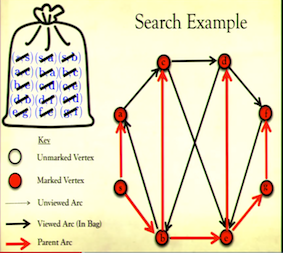
\includegraphics{lecture81}
\end{center}
\item Running Time:
	\begin{itemize}
	\item We search each arc out of v only once, when v is first marked.
	\item The arc is then added to the bag once and later removed from the bag once.
	\item Runtime = $O(m)$
	\item Linear time algorithm.
	\end{itemize}
\item Validity
	
 \textbf{Theorem.} Let G be a connected, undirected graph. Then the search algorithm finds every vertex in G.\\
 \textbf{Proof.}
 	\begin{itemize}
	\item We must show that each vertex v is  \textbf{marked} by the search algorithm.
	\item We prove this by induction on the smallest number k of edges in a path from the vertex to the root.
	\end{itemize}
\underline{Base Case:} k = 0
	\begin{itemize}
	\item Then v is the root vertex r.
	\item But r is the first vertex marked in the algorithm, so the base case holds.
	\end{itemize}
	
\underline{Induction Hypothesis:} 
	\begin{itemize}
	\item Assume any vertex v that has a path of (k - 1) (or fewer) edges to the root r is marked.
	\end{itemize}
	
\underline{Induction Step:} 
	\begin{itemize}
	\item Assume there is a path P with k edges from $v_k$ to r. Specifically let
	$$ P = \{v = v_k, v_{k-1}, ... , v_1, v_0 = r\}$$
	\item Thus there is a path Q with (k - 1) edges from $u = v_{k - 1} $ to r. That is. 
	$$ Q = \{u = v_{k-1}, ... , v_1, v_0 = r\}$$
	\item So, by the induction hypothesis, the vertex u is marked.
	\item After we mark u, we place the edges incident to it in the bag,
		\begin{itemize}
		\item The edge (u, v) is added to the bag.
		\end{itemize}
	\item Thus, when (u, v) is removed from the bag we will mark v. (If it is not already marked.)
	\end{itemize}
	
\item Validity in Directed Graphs
	\begin{itemize}
	\item For directed graphs, a similar argument proves that each vertex that has a directed path to it from the root r is \textbf{marked.}
	\end{itemize}
\end{itemize}


\section{Search Tree}
\renewcommand{\labelitemii}{$\circ$}
\renewcommand{\labelitemiii}{$\cdot$}
\renewcommand{\labelitemiii}{$\rightarrow$}
\renewcommand{\labelitemiv}{$\star$}
\begin{itemize}
\item Observe that each non-root vertex has exactly one predecessor.\\
 \textbf{Theorem.} Let G be a connected, undirected graph. Then the predecessor edges form a tree rooted at r.\\
 \textbf{Proof.}
	 \begin{itemize}
	\item By induction on the number of k of marked vertices.
	\end{itemize}
\underline{Base Case:} k = 1
	\begin{itemize}
	\item Then v is the first vertex marked.
		\begin{itemize}
		\item So the base case holds.
		\end{itemize}
	\end{itemize}
	
\underline{Induction Hypothesis:} 
	\begin{itemize}
	\item Assume the predecessor edges for the first (k -1) marked vertices form a tree rooted at r.
	\end{itemize}
	
\underline{Induction Step:} 
	\begin{itemize}
	\item Let v be the kth vertex to be marked.
	\item Assume v was marked when we removed the edge (u, v).
		\begin{itemize}
		\item $u = p(v)$
		\end{itemize}
	\item But (u, v) was added to the bag when we marked vertex u.
		\begin{itemize}
		\item Vertex u is in the set S of the first (k - 1) vertices to be marked.
		\end{itemize}
	\item By the induction hypothesis, the predecessor edges for S form a tree T rooted at r.
	\item $T \cup (p(v), v)$ is a tree rooted at r on the first k marked vertices.
	\end{itemize}
\end{itemize}



\section{Inplementational Aspects}
\renewcommand{\labelitemii}{$\circ$}
\renewcommand{\labelitemiii}{$\cdot$}
\renewcommand{\labelitemiii}{$\rightarrow$}
\renewcommand{\labelitemiv}{$\star$}
\begin{itemize}
\item There is some flexibility in how to implement the search algorithm?
	\begin{itemize}
	\item If the bag contains many arcs, which one should we remove?
	\end{itemize}
\item In fact, what in computer science is a "bag"?
\item The "bag" is just short-hand for a data structure.
\item Moreover, the choice of data structure used has important consequences.
\item Three choices of data structure for the bag give fundamental algorithms:
	\begin{itemize}
	\item Queue: Breadth First Search
	\item Stack: Depth First Search
	\item Priority Queue: Minimum Spanning Tree Algorithm
	\end{itemize}
\end{itemize}


\section{Breadth First Search}
\renewcommand{\labelitemii}{$\circ$}
\renewcommand{\labelitemiii}{$\cdot$}
\renewcommand{\labelitemiii}{$\rightarrow$}
\renewcommand{\labelitemiv}{$\star$}
\begin{itemize}
\item Using a \textbf{Queue} (FIFO) data structure produces:\\
\underline{Breadth First Search Algorithm}\\
Add (*, r) to a Queue\\
\forceindent \textbf{While} the Queue is non-empty\\
\forceindent \forceindent Remove the first arc (u, v) from the Queue\\
\forceindent \forceindent If v is unmarked \\
\forceindent \forceindent \forceindent Mark v\\
\forceindent \forceindent \forceindent Set $p(v) \leftarrow u$ \\ 
\forceindent \forceindent \forceindent For each arc(v,w)\\
\forceindent \forceindent \forceindent \forceindent Add (v, w) into the back of the Queue
\end{itemize}
\begin{center}
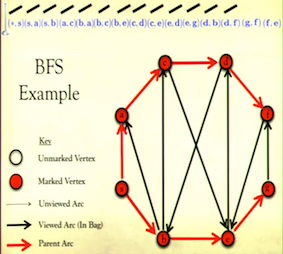
\includegraphics{lecture82}
\end{center}


\section{Breadth First Search Trees}
\renewcommand{\labelitemii}{$\circ$}
\renewcommand{\labelitemiii}{$\cdot$}
\renewcommand{\labelitemiii}{$\rightarrow$}
\renewcommand{\labelitemiv}{$\star$}
\begin{itemize}
\item Because BFS uses a queue it is easy to verify that:
	\begin{itemize}
	\item The edges are added to the queue in order of their distance from r/
	\item The vertices are marked in order of their distance from r.
	\end{itemize}
\item Specifically:\\
\textbf{Theorem.} For any vertex v, the path from v to r given by the search tree T of predecessor edges is a shortest path.\\
Exercise: Verify this formally.
\item Structure:
	\begin{itemize}
	\item Let $S_l$ be the set or "layer" of vertices at distance $l$ from r in T.
	\item Then a vertex $v \in S_l$ is also at distance $l$ from r in the whole graph G.
		\begin{itemize}
		\item Thus implies for every non-tree edge (u, v), u and v are either in the same layer or in adjacent layers.
		\item If not, we can find a shorter path to the root from u or v.
		\end{itemize}
	\end{itemize}
\end{itemize}
\begin{center}
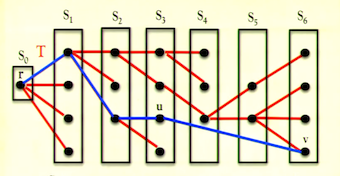
\includegraphics{lecture83}
\end{center}


\section{BFS and Bipartite Graphs}
\renewcommand{\labelitemii}{$\circ$}
\renewcommand{\labelitemiii}{$\cdot$}
\renewcommand{\labelitemiii}{$\rightarrow$}
\renewcommand{\labelitemiv}{$\star$}
\begin{itemize}
\item Recall in a \textbf{bipartite graph} the vertex set can be partitioned as $V = X \cup Y$ such that every edge has one end-vertex in $X$ and one end-vertex in $Y$.\\

\textbf{Theorem.}  A graph G is bipartite if and only if it contains no odd length cycles.\\
\textbf{Proof.}\\
($\Rightarrow$)
	\begin{itemize}
	\item Assume G contains as a subgraph an odd length cycle C.
	\item let $C = \{v_0, v_1, v_2, ... , v_{2k} \}$
	\item Wlog we may assume vertex $v_0 \in Y$. Therefore:\\
	$$v_0 \in Y \Rightarrow v_1 \in Y \Rightarrow \cdot \cdot \cdot \Rightarrow v_{2k} \in Y$$
	\item But $(v_0, v_{2k}) \in E $. Thus\\
	$$v_0 \in Y \Rightarrow  v_{2k} \in Y$$
	\\
	\\
	\end{itemize}
\begin{center}
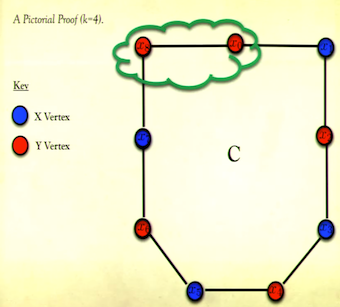
\includegraphics{lecture84}
\end{center}

($\Leftarrow$)
	\begin{itemize}
	\item Assume G contains no odd length cycles.
	\item Select an arbitrary root vertex r and run the BFS algorithm.
	\item Recall that for every non-tree edge (u, v), u and v are either in the same layer or in adjacent layers.
	\item Now set: 
	\[
 X = \bigcup_{l\;odd}^{} S_{l} \; \; \;
 Y = \bigcup_{l\;even}^{} S_{l}
\]
	
	\item Suppose, for every non-tree edge (u, v), that u and v are in adjacent layers.
	\item Now, for every tree edge (u, v) we also have u and v in adjacent layers.
	\item So assume, there is non-tree edge (u, v) with u and v in the same layer.
	\item Let z be the closest common ancestor of u and v in the search tree T.
	\item Let P be the path in T from u to z; let Q be the path in T from v to z.
	\item Since u and v in the same layer we have: $|P| = |Q|$
	\item But then the cycle $C = P \cup Q \cup (u,v) $ has an odd number of edges as:
	
	\end{itemize}
\end{itemize}
\begin{center}
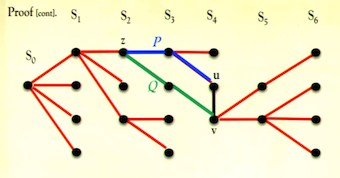
\includegraphics{lecture85}
\end{center}










\end{document}